\chapter{Katalyse}\label{ch:g12:catalysis}

Een fles waterstofperoxide staat maandenlang onveranderd in een
badkamerkastje. Op een geschaafde knie gegoten schuimt ze meteen: iets in
het bloed laat het in een paar seconden ontleden in water en zuurstof.
Dat iets wordt niet verbruikt, en het staat niet in de vergelijking van
de reactie. Het is een \omterm{def:g12:catalysis:catalyst}{katalysator}. \omterm{def:g12:catalysis:catalyst}{Katalysatoren} maken het grootste deel
van de chemische industrie mogelijk, reinigen de uitlaatgassen van auto's
en sturen elke reactie van het leven.

\begin{recall}
De snelheid van een reactie en de \omterm{def:g12:reaction-rates:kinetic-factor}{kinetische factoren} die haar veranderen
(\cref{ch:g12:reaction-rates}). Een mechanisme is een reeks \omterm{def:g12:curly-arrows:mechanism}{elementaire
stappen}, via intermediairen (\cref{ch:g12:curly-arrows}).
\end{recall}

\section{Wat een katalysator is}

\begin{definition}[Katalysator, katalyse]\label{def:g12:catalysis:catalyst}
Een \emph{katalysator}\index{katalysator} is een deeltje dat een reactie
sneller maakt zonder verbruikt te worden: het doet mee aan het mechanisme,
maar wordt aan het eind onveranderd teruggegeven, en het staat niet in de
totale \omterm{def:g8:balanced-equations:equation}{reactievergelijking}. Het versnellen van een reactie door een
katalysator heet \emph{katalyse}\index{katalyse}.
\end{definition}

\begin{proposition}[Een katalysator verandert de weg, niet de bestemming]\label{prop:g12:catalysis:path}
Een \omterm{def:g12:catalysis:catalyst}{katalysator} opent een ander mechanisme, met lagere energiebarrières
dan die van de niet-gekatalyseerde reactie, zodat meer ontmoetingen
tussen deeltjes slagen. Hij verandert niet welke \omterm{def:g7:chemical-reactions:reactant}{reactieproducten}
ontstaan, en ook niet welke \omterm{def:g10:reaction-progress-table:system}{eindtoestand} bereikt wordt; hij bereikt die
alleen sneller.
\end{proposition}

\begin{proof}
Aangenomen: het energieprofiel wordt bestudeerd in het deel voor het
eerste universiteitsjaar. Dat de \omterm{def:g10:reaction-progress-table:system}{eindtoestand} niet verandert, volgt
daaruit dat de \omterm{def:g12:catalysis:catalyst}{katalysator} wordt teruggegeven: de totale reactie,
\omterm{def:g7:chemical-reactions:reactant}{beginstoffen} en \omterm{def:g7:chemical-reactions:reactant}{reactieproducten}, is dezelfde.
\end{proof}

\begin{omfigure}
\begin{minipage}{0.49\linewidth}
\begin{tikzpicture}
\begin{axis}[width=\linewidth, height=5.4cm, xmin=0, xmax=1, ymin=-60,
    ymax=110, xtick=\empty, ytick=\empty, axis lines*=left,
    xlabel={voortgang van de reactie}, ylabel={energie},
    label style={font=\small}, legend style={font=\scriptsize,
    at={(0.02,0.99)}, anchor=north west, draw=none}, legend cell align=left]
  \addplot[very thick, omDef] table[x=s, y=Eu] {figdata/out/grade-12-catalysis-a.dat};
  \addplot[very thick, omProp] table[x=s, y=Ec] {figdata/out/grade-12-catalysis-a.dat};
  \legend{zonder katalysator, met katalysator}
  \node[font=\scriptsize, anchor=north west] at (axis cs:0.02,-4) {beginstoffen};
  \node[font=\scriptsize, anchor=south east] at (axis cs:0.99,-36) {producten};
\end{axis}
\end{tikzpicture}
\end{minipage}\hfill
\begin{minipage}{0.49\linewidth}
\begin{tikzpicture}
\begin{axis}[width=\linewidth, height=5.4cm, xmin=0, xmax=60, ymin=0,
    ymax=80, xlabel={$t$ (\si{min})}, ylabel={vrijgekomen \ce{O2} (\si{mL})},
    axis lines*=left, ymajorgrids, grid style={gray!20},
    tick label style={font=\scriptsize}, label style={font=\small},
    legend style={font=\scriptsize, at={(0.98,0.03)}, anchor=south east,
    draw=none}, legend cell align=left]
  \addplot[very thick, omDef] table[x=t, y=Vu] {figdata/out/grade-12-catalysis-b.dat};
  \addplot[very thick, omProp] table[x=t, y=Vc] {figdata/out/grade-12-catalysis-b.dat};
  \legend{zonder katalysator, met katalysator}
\end{axis}
\end{tikzpicture}
\end{minipage}

{\small Links: de energie langs de reactie; de gekatalyseerde weg loopt
via een intermediair en twee lagere barrières. Rechts: de zuurstof die
vrijkomt uit een oplossing van waterstofperoxide; de \omterm{def:g12:catalysis:catalyst}{katalysator}
versnelt de reactie, maar het eindvolume is hetzelfde. (Modelkrommen.)}
\end{omfigure}

\section{Homogene katalyse}

\begin{definition}[Homogene en heterogene katalyse]\label{def:g12:catalysis:homogeneous}
Er is sprake van \emph{homogene katalyse}\index{homogene katalyse}
als de \omterm{def:g12:catalysis:catalyst}{katalysator} in dezelfde fase is als de \omterm{def:g7:chemical-reactions:reactant}{beginstoffen} (bijvoorbeeld
samen met ze opgelost), en van \emph{heterogene katalyse}\index{heterogene katalyse}
als hij in een andere fase is, meestal een vaste stof waarvan de
\omterm{def:g7:chemical-reactions:reactant}{beginstoffen} het oppervlak bereiken vanuit een gas of een vloeistof.
\end{definition}

\begin{example}[Jodide-ionen en waterstofperoxide]\label{ex:g12:catalysis:iodide}
Waterstofperoxide ontleedt uit zichzelf heel langzaam:
\ce{2H2O2 -> 2H2O + O2}. Met een beetje kaliumjodide erin opgelost begint
het meteen te schuimen. Het \omterm{def:g9:ions:ion}{jodide-ion} opent een weg in twee stappen:
\[
  \ce{H2O2 + I- -> H2O + IO-}, \qquad
  \ce{H2O2 + IO- -> H2O + O2 + I-} .
\]
Opgeteld geven de twee stappen weer \ce{2H2O2 -> 2H2O + O2}: het
\omterm{def:g9:ions:ion}{jodide-ion}, dat in de eerste stap gebruikt en in de tweede teruggegeven
wordt, is de \omterm{def:g12:catalysis:catalyst}{katalysator}; het \omterm{def:g9:ions:ion}{ion} \ce{IO-} is een intermediair.
\end{example}


\begin{example}[IJzer(III)ionen]\label{ex:g12:catalysis:iron}
Ook ijzer(III)\omterm{def:g9:ions:ion}{ionen} katalyseren de ontleding, via het koppel
\ce{Fe^{3+}}/\ce{Fe^{2+}} (\cref{ch:g11:redox}): eerst oxideren ze
waterstofperoxide, \ce{2Fe^{3+} + H2O2 -> 2Fe^{2+} + O2 + 2H+}, daarna
worden de gevormde ijzer(II)\omterm{def:g9:ions:ion}{ionen} door meer waterstofperoxide weer
geoxideerd, \ce{2Fe^{2+} + H2O2 + 2H+ -> 2Fe^{3+} + 2H2O}. De lichtoranje
kleur van de oplossing wordt groenig zolang het gas vrijkomt, en komt
terug als het waterstofperoxide op is: een teken dat de \omterm{def:g12:catalysis:catalyst}{katalysator}
meedoet en weer terugkomt.
\end{example}

\section{Heterogene katalyse}

Veel industriële \omterm{def:g12:catalysis:catalyst}{katalysatoren} zijn vaste stoffen: \omterm{def:g9:periodic-table-first-look:metal}{metalen} zoals platina,
palladium, nikkel of ijzer, of oxiden. De reactie vindt plaats aan hun
oppervlak, in drie fasen: de \omterm{def:g7:atoms-and-molecules:molecule}{moleculen} van de \omterm{def:g7:chemical-reactions:reactant}{beginstoffen} worden aan het
oppervlak vastgehouden (geadsorbeerd), waar hun bindingen verzwakt worden;
ze reageren daar; de \omterm{def:g7:chemical-reactions:reactant}{reactieproducten} verlaten het oppervlak, dat weer vrij
is voor nieuwe \omterm{def:g7:atoms-and-molecules:molecule}{moleculen}. Een \omterm{def:g12:catalysis:catalyst}{katalysator} wordt daarom gemaakt met een zo
groot mogelijk oppervlak: een fijn poeder, of een dun laagje op een poreuze
drager.

\begin{omfigure}
\begin{tikzpicture}[font=\small]
  \foreach \x in {0,4.2,8.4} {
    \fill[black!25] (\x,0) rectangle (\x+3.4,0.35);
    \foreach \i in {0,1,2,3,4,5,6,7} \shade[ball color=black!35] (\x+0.21+\i*0.425,0.35) circle (0.2);
  }
  % 1. adsorption
  \node[aH, minimum size=3.2mm] at (0.9,0.75) {};
  \node[aH, minimum size=3.2mm] at (1.3,0.75) {};
  \node[aH, minimum size=3.2mm] (h1) at (2.2,1.8) {};
  \node[aH, minimum size=3.2mm] (h2) at (2.6,1.8) {};
  \draw[bond, line width=1.2pt] (h1.east) -- (h2.west);
  \draw[->, omProp, thick] (2.4,1.55) -- (2.0,1.0);
  \node[anchor=north, align=center] at (1.7,-0.1) {1. geadsorbeerd:\\ de \ce{H-H}-binding breekt};
  % 2. reactie aan het oppervlak
  \node[aC] (c1) at (5.5,1.05) {}; \node[aC] (c2) at (6.2,1.05) {};
  \draw[bond, line width=1.4pt] (c1) -- (c2);
  \node[aH, minimum size=3.2mm] at (5.3,0.75) {};
  \node[aH, minimum size=3.2mm] at (6.6,0.75) {};
  \node[anchor=north, align=center] at (5.9,-0.1) {2. de H-atomen binden aan\\ het geadsorbeerde molecuul};
  % 3. desorptie
  \node[aC] (c3) at (9.6,1.8) {}; \node[aC] (c4) at (10.3,1.8) {};
  \draw[bond, line width=1.4pt] (c3) -- (c4);
  \foreach \a/\c in {150/c3,210/c3,90/c3,30/c4,-30/c4,90/c4}
    \node[aH, minimum size=2.8mm] at ($(\c)+(\a:0.42)$) {};
  \draw[->, omProp, thick] (11.0,1.2) -- (11.0,2.2);
  \node[anchor=north, align=center] at (10.1,-0.1) {3. het product\\ verlaat het oppervlak};
\end{tikzpicture}

{\small Waterstof dat aan etheen addeert op een metaaloppervlak: adsorptie,
reactie, desorptie. Het \omterm{def:g9:periodic-table-first-look:metal}{metaal} wordt onveranderd teruggegeven.}
\end{omfigure}

\begin{example}[De uitlaatkatalysator]\label{ex:g12:catalysis:converter}
In de uitlaatgassen van een benzinemotor zitten twee giftige gassen,
koolstofmono-oxide en stikstofmono-oxide, en onverbrande
\omterm{def:g4:what-a-fire-needs:fuel}{brandstof}. In de uitlaatkatalysator,
een keramische honingraat bedekt met platina en rodium, reageren ze aan
het metaaloppervlak:
\[
  \ce{2CO + 2NO -> 2CO2 + N2} ,
\]
en de koolwaterstoffen \omterm{def:g4:what-a-fire-needs:burning}{verbranden} tot koolstofdioxide en water. De gassen
gaan in een fractie van een seconde door de \omterm{def:g12:catalysis:catalyst}{katalysator}, te snel voor
welke reactie dan ook zonder \omterm{def:g12:catalysis:catalyst}{katalysator}.
\end{example}

\begin{omfigure}
\begin{tikzpicture}[font=\small]
  \fill[black!12, draw=black!60, rounded corners=6pt] (0,0) rectangle (6,2.4);
  \foreach \x in {0.3,0.6,0.9,1.2,1.5,1.8,2.1,2.4,2.7,3.0,3.3,3.6,3.9,4.2,4.5,4.8,5.1,5.4,5.7} \draw[black!35] (\x,0.2) -- (\x,2.2);
  \foreach \y in {0.5,0.9,1.3,1.7,2.1} \draw[black!35] (0.2,\y) -- (5.8,\y);
  \fill[black!40] (-1.4,0.9) rectangle (0,1.5);
  \fill[black!40] (6,0.9) rectangle (7.4,1.5);
  \draw[->, very thick, omThm] (-2.6,1.2) -- (-1.5,1.2);
  \node[anchor=east, align=right, omThm] at (-2.7,1.2) {\ce{CO}, \ce{NO},\\ koolwaterstoffen};
  \draw[->, very thick, omMeth] (7.5,1.2) -- (8.6,1.2);
  \node[anchor=west, align=left, omMeth] at (8.7,1.2) {\ce{CO2}, \ce{N2},\\ \ce{H2O}};
  \node[align=center, fill=white, inner sep=2pt] at (3,1.2) {keramische honingraat\\ bedekt met Pt en Rh};
\end{tikzpicture}

{\small Een uitlaatkatalysator, in de lengte doorgesneden: duizenden dunne
kanaaltjes geven de uitlaatgassen een enorm oppervlak met een laagje
\omterm{def:g9:periodic-table-first-look:metal}{metaal}.}
\end{omfigure}

\begin{omfigure}
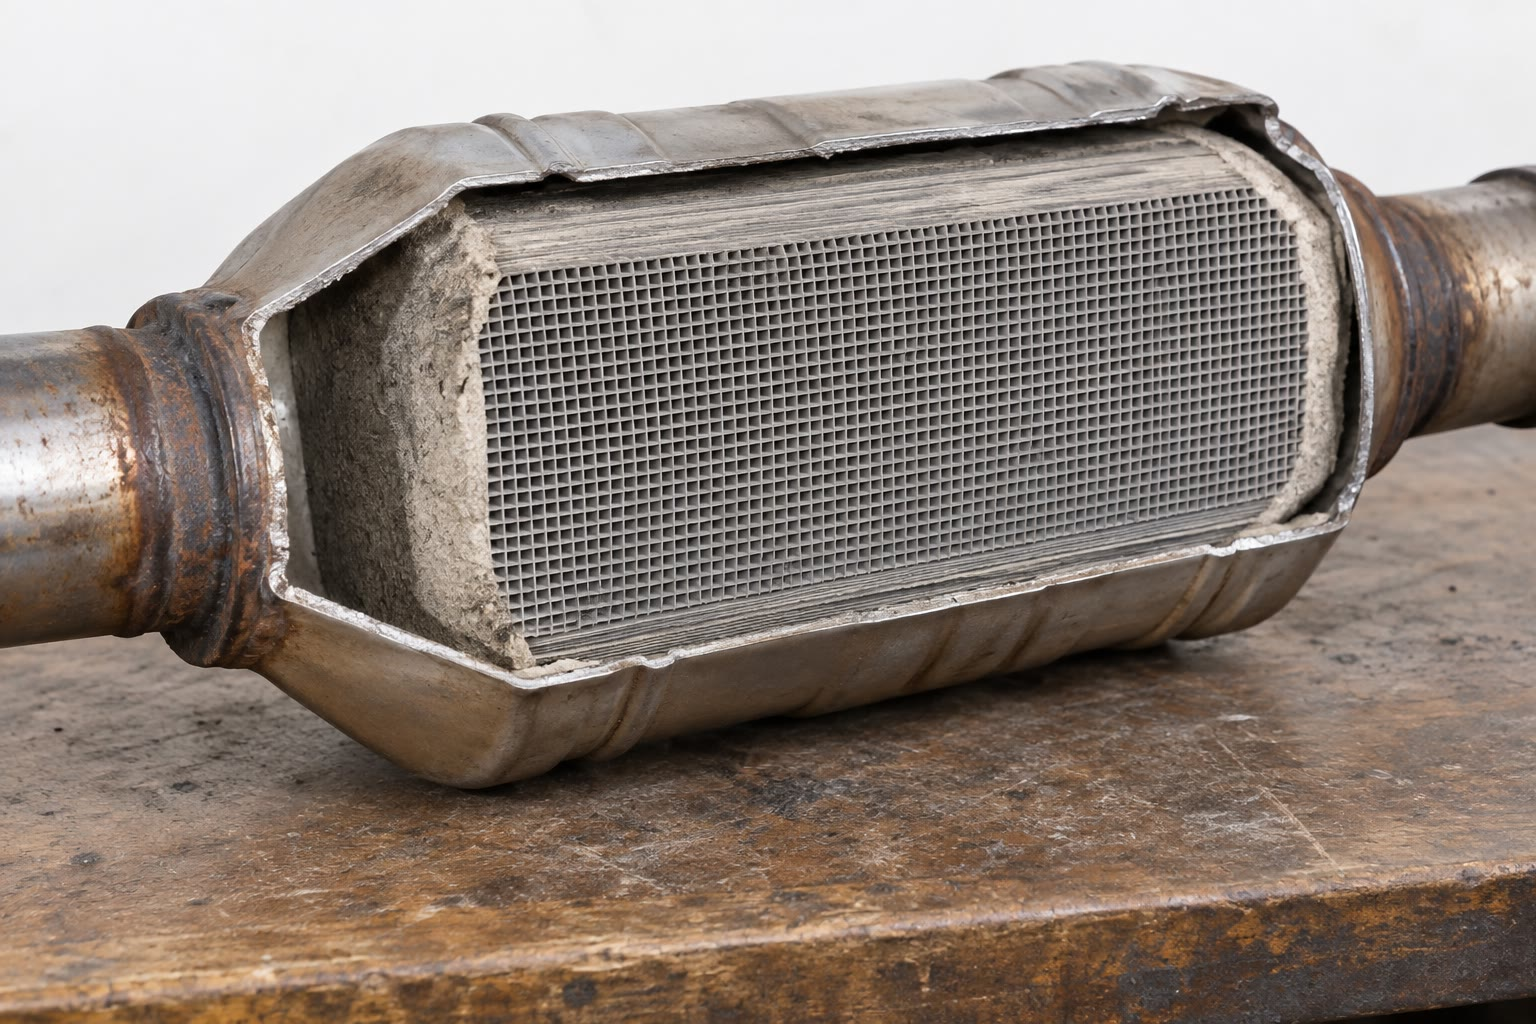
\includegraphics[width=0.45\linewidth]{images/book1/ai/g12-catalytic-converter.jpg}

{\small Een opengezaagde uitlaatkatalysator: de kern van honingraat.}
\end{omfigure}

\begin{history}[Haber, Bosch en ammoniak]
% ledger: haber:T, haber:p, nh3:world-2024
Aan het begin van de twintigste eeuw vond de scheikundige Fritz Haber hoe
je de stikstof uit de \omterm{def:g4:air-a-mixture-of-gases:air}{lucht} met waterstof kunt laten reageren,
\ce{N2 + 3H2 -> 2NH3}, op een \omterm{def:g12:catalysis:catalyst}{katalysator} op basis van ijzer, en de
ingenieur Carl Bosch maakte er een industrieel proces van. Het draait nog
steeds, bij 400
tot \qty{500}{\celsius} en 150 tot \qty{250}{atm}. In 2024 maakte de
wereld ammoniak met daarin ongeveer 150 miljoen ton stikstof, het meeste
voor kunstmest: een groot deel van de stikstof in het voedsel dat we eten,
is door zo'n \omterm{def:g12:catalysis:catalyst}{katalysator} gegaan.
\end{history}

\section{Enzymen}

\begin{definition}[Enzym]\label{def:g12:catalysis:enzyme}
Een \emph{enzym}\index{enzym} is een eiwit dat door een levend organisme
gemaakt wordt en dat één reactie van zijn chemie katalyseert. Enzymen zijn
zeer efficiënt en zeer specifiek: elk past maar op een paar \omterm{def:g7:atoms-and-molecules:molecule}{moleculen}, en
ze werken het best binnen een smal gebied van temperatuur en zuurgraad.
\end{definition}

\begin{example}[Katalase]\label{ex:g12:catalysis:catalase}
Waterstofperoxide ontstaat in cellen als bijproduct, en is schadelijk
voor ze. Het \omterm{def:g12:catalysis:enzyme}{enzym} katalase, dat in bloed, lever en veel plantenweefsels
voorkomt, ontleedt het met enorme snelheid in water en zuurstof: dat is
het schuim op een geschaafde knie, of op een plakje rauwe aardappel.
Gekookte aardappel geeft geen schuim: het verwarmen heeft de vorm van het
\omterm{def:g12:catalysis:enzyme}{enzym} vernietigd.
\end{example}

\begin{omfigure}
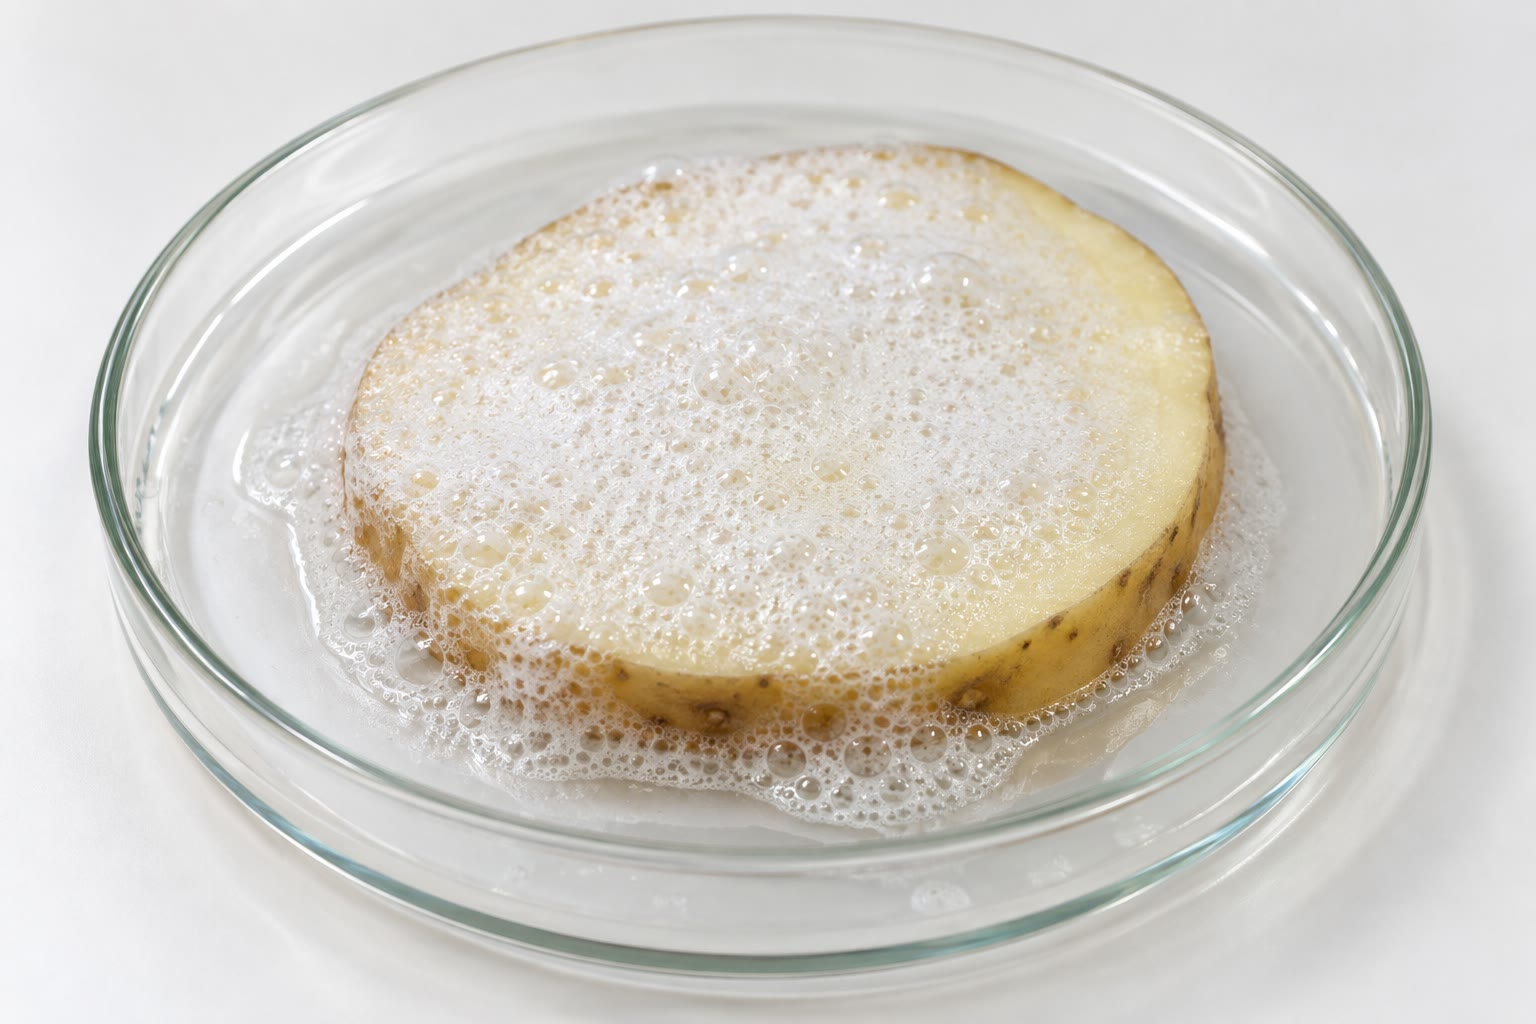
\includegraphics[width=0.45\linewidth]{images/book1/ai/g12-potato-peroxide.jpg}

{\small Waterstofperoxide op een plakje rauwe aardappel: katalase aan het
werk.}
\end{omfigure}

\section{Selectiviteit}

\begin{definition}[Selectieve katalysator]\label{def:g12:catalysis:selective}
Als dezelfde \omterm{def:g7:chemical-reactions:reactant}{beginstoffen} verschillende reacties kunnen geven, versnelt
een \emph{selectieve katalysator}\index{selectieve katalysator} er één
veel meer dan de andere, en bepaalt hij zo welke \omterm{def:g7:chemical-reactions:reactant}{reactieproducten}
ontstaan.
\end{definition}

\begin{example}[Twee lotgevallen van ethanol]\label{ex:g12:catalysis:ethanol}
Hete ethanoldamp die over aluminiumoxide wordt geleid, verliest water en
geeft etheen, \ce{C2H5OH -> C2H4 + H2O} (een \omterm{def:g12:curly-arrows:categories}{eliminatie}); over heet koper
geleid verliest ze waterstof en geeft ze ethanal,
\ce{C2H5OH -> CH3CHO + H2}. Dezelfde \omterm{def:g7:chemical-reactions:reactant}{beginstof}, twee \omterm{def:g12:catalysis:catalyst}{katalysatoren}, twee
\omterm{def:g7:chemical-reactions:reactant}{reactieproducten}.
\end{example}

\begin{remark}[Industrie en leven draaien op katalysatoren]\label{rem:g12:catalysis:everywhere}
De meeste producten van de chemische industrie, van \omterm{def:g4:what-a-fire-needs:fuel}{brandstoffen} tot
\omterm{def:g8:plastics:plastic}{kunststoffen} en kunstmest, worden met \omterm{def:g12:catalysis:catalyst}{katalysatoren} gemaakt; een
actievere of selectievere \omterm{def:g12:catalysis:catalyst}{katalysator} vinden spaart energie en afval.
Elke reactie in een levende cel wordt door een \omterm{def:g12:catalysis:enzyme}{enzym} gekatalyseerd.
\end{remark}

\begin{safety}{\ghs[0.82cm]{GHS03}\ghs[0.82cm]{GHS05}\ghs[0.82cm]{GHS07}}
% ledger: ghs:H2O2
Geconcentreerd waterstofperoxide is een sterke \omterm{def:g11:redox:oxidant}{oxidator} die een brand kan
aanwakkeren, het brandt huid en ogen, en het is schadelijk bij inslikken.
Ook de verdunde oplossingen van het laboratorium vragen om een
veiligheidsbril en handschoenen; bij de ontleding komt zuurstof vrij, dus
ze wordt nooit in een gesloten vat uitgevoerd.
\end{safety}

\section{Oefeningen}


\begin{exercise}[$\star$]\label{exo:g12:catalysis:1}
Welke deeltjes zijn bij de ontleding van waterstofperoxide, gekatalyseerd
door \omterm{def:g9:ions:ion}{jodide-ionen}, \omterm{def:g7:chemical-reactions:reactant}{beginstoffen}, welke \omterm{def:g7:chemical-reactions:reactant}{reactieproducten}, welk is de
\omterm{def:g12:catalysis:catalyst}{katalysator} en welk een intermediair?
\end{exercise}

\begin{exercise}[$\star$]\label{exo:g12:catalysis:2}
Homogene of \omterm{def:g12:catalysis:homogeneous}{heterogene katalyse}: \omterm{def:g9:ions:ion}{jodide-ionen} in een oplossing van
waterstofperoxide; platina in een uitlaatkatalysator; ijzer bij de
ammoniaksynthese; ijzer(III)\omterm{def:g9:ions:ion}{ionen} in een oplossing van waterstofperoxide?
\end{exercise}

\begin{exercise}[$\star$]\label{exo:g12:catalysis:3}
Welke weg heeft in de energieprofielen de hoogste barrière? Zijn de
begin- en eindenergie op beide wegen dezelfde? Wat betekent dit voor de
\omterm{def:g7:chemical-reactions:reactant}{reactieproducten}?
\end{exercise}

\begin{exercise}[$\star$]\label{exo:g12:catalysis:4}
Waarom staat een \omterm{def:g12:catalysis:catalyst}{katalysator} niet in de totale \omterm{def:g8:balanced-equations:equation}{reactievergelijking} van een
reactie?
\end{exercise}

\begin{exercise}[$\star$]\label{exo:g12:catalysis:5}
Waarom worden de vaste \omterm{def:g12:catalysis:catalyst}{katalysatoren} van de industrie gebruikt als fijn
poeder of als dun laagje op een poreuze drager?
\end{exercise}

\begin{exercise}[$\star\star$]\label{exo:g12:catalysis:6}
Tel de twee stappen op van de door ijzer(III) gekatalyseerde ontleding van
waterstofperoxide, en laat zien dat de ijzerionen en de waterstofionen
wegvallen.
\end{exercise}

\begin{exercise}[$\star\star$]\label{exo:g12:catalysis:7}
Lees de krommen van de vrijgekomen zuurstof af. Hoe lang duurt het bij
elke proef tot de helft van het eindvolume is vrijgekomen? Met welke
factor verkort de \omterm{def:g12:catalysis:catalyst}{katalysator} die tijd?
\end{exercise}

\begin{exercise}[$\star\star$]\label{exo:g12:catalysis:8}
Gelode benzine wordt niet gebruikt in auto's met een uitlaatkatalysator:
het lood zet zich op het platina af en blijft daar. Leg uit waarom dit de
\omterm{def:g12:catalysis:catalyst}{katalysator} ruïneert, hoewel het platina bij de normale reactie niet
verbruikt wordt.
\end{exercise}

\begin{exercise}[$\star\star$]\label{exo:g12:catalysis:9}
Een leerling meet het schuim dat plakjes aardappel in waterstofperoxide
geven bij 10, 25, 37, 60 en \qty{80}{\celsius}: het schuim neemt toe tot
ongeveer \qty{37}{\celsius}, neemt dan af, en verdwijnt bijna bij
\qty{80}{\celsius}. Verklaar beide delen van de kromme.
\end{exercise}

\begin{exercise}[$\star\star$]\label{exo:g12:catalysis:10}
Schrijf de vergelijking op van de reactie in een uitlaatkatalysator tussen
koolstofmono-oxide en stikstofmono-oxide, en controleer dat ze klopt.
Waarom verdwijnen beide verontreinigingen tegelijk?
\end{exercise}

\begin{exercise}[$\star\star$]\label{exo:g12:catalysis:11}
\qty{10.0}{mL} oplossing van waterstofperoxide geeft bij volledige
ontleding \qty{72}{mL} zuurstof bij \qty{20}{\celsius}. Bereken de
hoeveelheid zuurstof ($V_m = \qty{24.1}{L/mol}$), en daarna de
concentratie waterstofperoxide van de oplossing.
\end{exercise}

\begin{exercise}[$\star\star\star$]\label{exo:g12:catalysis:12}
Ethanoldamp die over aluminiumoxide wordt geleid, geeft etheen; over koper
geeft ze ethanal. Schrijf beide vergelijkingen op, geef aan tot welke
soort de eerste behoort, en leg uit wat een \omterm{def:g12:catalysis:selective}{selectieve katalysator} is.
\end{exercise}

\begin{exercise}[$\star\star\star$]\label{exo:g12:catalysis:13}
Een \omterm{def:g12:catalysis:catalyst}{katalysator} maakt een reactie tien keer sneller. Een leerling beweert
dat hij ook tien keer zoveel product geeft. Verbeter die bewering met de
krommen van de vrijgekomen zuurstof.
\end{exercise}

\begin{exercise}[$\star\star\star$]\label{exo:g12:catalysis:14}
Eén \omterm{def:g7:atoms-and-molecules:molecule}{molecuul} katalase ontleedt ongeveer een paar miljoen \omterm{def:g7:atoms-and-molecules:molecule}{moleculen}
waterstofperoxide per seconde. Neem $\num{5e6}$ per seconde: hoe lang doet
één enzymmolecuul erover om één \omterm{def:g10:the-mole:amount}{mol} waterstofperoxide te ontleden? Hoeveel
enzymmoleculen zouden het in één seconde doen? (Een berekening in ordes
van grootte; de snelheid is een gegeven van de oefening.)
\end{exercise}

\begin{exercise}[$\star\star\star$]\label{exo:g12:catalysis:15}
% ledger: nh3:world-2024
De wereld maakte in 2024 ongeveer 150 miljoen ton stikstof in de vorm van
ammoniak. Welke massa ammoniak is dat? Welke hoeveelheid stikstofgas
werd er gebonden?
\end{exercise}

\section{Probleem: Het waterstofperoxide van de kapper}

\begin{problem}[{Weekendprobleem --- wat is de concentratie van
waterstofperoxide van ``20 volumes''?}]
\label{pb:g12:catalysis:1}
% ledger: const:Vm1, ghs:H2O2, aw:H, aw:O
Kappers gebruiken oplossingen van waterstofperoxide waarvan de sterkte in
``volumes'' op het etiket staat: een oplossing van ``20 volumes'' is een
oplossing waarvan \qty{1}{L} bij volledige ontleding \qty{20}{L} zuurstof
geeft, gemeten bij \qty{0}{\celsius} en normale luchtdruk, waar één \omterm{def:g10:the-mole:amount}{mol}
gas \qty{22.4}{L} inneemt.

\medskip
\noindent\textbf{Deel I --- De ontleding.}
\begin{enumerate}
  \item Schrijf de vergelijking op van de ontleding van waterstofperoxide.
  \item Is de ontleding een \omterm{def:g11:redox:reaction}{redoxreactie}? Zoek de \omterm{def:g11:redox:oxidant}{oxidator} en de \omterm{def:g11:redox:oxidant}{reductor}
        (waterstofperoxide is allebei).
  \item Waarom blijft een fles maandenlang goed, hoewel de reactie
        mogelijk is?
\end{enumerate}

\medskip
\noindent\textbf{Deel II --- Wat ``20 volumes'' betekent.}
\begin{enumerate}[resume]
  \item Welke hoeveelheid zuurstof geeft \qty{1}{L} van de oplossing?
  \item Leid de hoeveelheid waterstofperoxide in \qty{1}{L} af.
  \item Geef de \omterm{def:g10:concentration-and-dilution:molar-concentration}{molaire concentratie}.
  \item Bereken de \omterm{def:g10:the-mole:molar-mass}{molaire massa} van waterstofperoxide en de
        \omterm{def:g10:concentration-and-dilution:mass-concentration}{massaconcentratie}.
  \item Wat zou ``10 volumes'' betekenen in \omterm{def:g10:the-mole:amount}{mol} per liter?
\end{enumerate}

\medskip
\noindent\textbf{Deel III --- Twee \omterm{def:g12:catalysis:catalyst}{katalysatoren}.}
\begin{enumerate}[resume]
  \item Een druppel bloed (katalase) en een paar druppels
        ijzer(III)chloride worden elk aan een monster toegevoegd. Welk
        soort \omterm{def:g12:catalysis:catalyst}{katalyse} is elk?
  \item Schrijf de twee stappen van de ijzer(III)\omterm{def:g12:catalysis:catalyst}{katalyse} op en controleer
        dat hun som de ontleding is.
  \item Beschrijf met de krommen van de vrijgekomen zuurstof hoe het
        volume zuurstof verandert met en zonder \omterm{def:g12:catalysis:catalyst}{katalysator}, en wat
        hetzelfde blijft.
  \item Waarom verandert de kleur van een monster met ijzer(III) als
        \omterm{def:g12:catalysis:catalyst}{katalysator} tijdens de reactie, en komt ze aan het eind terug?
  \item Waarom laat een gekookte aardappel de oplossing niet schuimen?
\end{enumerate}

\medskip
\noindent\textbf{Deel IV --- De fles.}
\begin{enumerate}[resume]
  \item Welk volume zuurstof, gemeten bij \qty{0}{\celsius}, kan een fles
        van \qty{100}{mL} afgeven?
  \item Welk volume is dat bij \qty{20}{\celsius} ($V_m =
        \qty{24.1}{L/mol}$)?
  \item Waarom moet de dop van zo'n fles langzaam gas laten ontsnappen?
  \item Een fles die lang bewaard is, wordt getitreerd en blijkt
        \qty{1.50}{mol/L} te bevatten. Hoeveel ``volumes'' is dat nu?
  \item Welk deel van het waterstofperoxide is ontleed?
  \item Geef het eindantwoord: wat is de \omterm{def:g10:concentration-and-dilution:molar-concentration}{molaire concentratie} van een
        oplossing van waterstofperoxide van ``20 volumes''?
\end{enumerate}
\end{problem}
